% ================================================================
\section{Introduction}
\label{sec:intro}
% ----------------------------------------------------------------
% ================================================================
Signal Temporal Logic (STL) is a standard formalism for specifying temporal
properties of real-valued signals~\cite{maler2004monitoring,fainekos2009robustness}.
Its quantitative \emph{robustness} semantics measures how strongly a behavior
satisfies or violates a specification, and underpins tasks in runtime
monitoring~\cite{bartocci2018survey}, falsification~\cite{annpureddy2011staliro},
and learning-enabled design~\cite{raman2014mpc}.

That semantics, though, is written for an idealized signal: continuous,
infinitely long, and defined at every instant. The signals an evaluator
actually receives are finite and sampled, and closing the gap demands
decisions the formula is silent about---how a signal behaves between two
samples, for instance, or what a temporal window sees past the last one. We
call these decisions \emph{implicit semantics}: they are absent from the STL
formula yet they shift the robustness value computed for it.

These decisions are easy to overlook, yet their consequences are not. Two
tools that resolve them differently can disagree on the same formula and the
same trace, with the difference tracing back to a silently adopted choice
rather than to anything the specification says---and a downstream search or
monitor runs to completion with no indication that its output rests on a
convention (\cref{sec:discrepancies}).

Existing tools reach evaluation through an application: a monitor, a falsifier,
or a learning library computes robustness as a means to its own end, and the
implicit choices are settled wherever that pipeline happens to settle them. We
take the opposite stance and treat evaluation itself as the object of interest.
\tool is built evaluation-first: the logical core of STL stays fixed behind a
stable interface, and the implicit choices live below it as explicit,
interchangeable backends rather than hard-coded assumptions.

Building a tool around evaluation rather than an application invites the
question of what it is good for. This paper makes the following contributions.
\begin{itemize}
  \item We identify STL robustness evaluation as a common but often implicit
    computational layer shared across monitoring, falsification, and related
    applications, and we organize its implicit choices into explicit
    decision points (\cref{sec:background}).
  \item We present \tool,%
    \footnote{\url{https://github.com/midoriao/tidystl}}
    a lightweight Python library that makes this layer explicit: formula
    structure, signal data, and evaluation are separated so that
    semantic choices attach as a switchable backend below a stable public API
    (\cref{sec:design}).
  \item We validate \tool with a systematic regression suite and a cross-tool
    comparison against Breach, RTAMT, and STLCG++.
    The comparison reveals that evaluator-level choices can cause observable discrepancies under the same nominal input
    (\cref{sec:discrepancies}).
  \item We show that representative robustness semantics can be expressed as
    localized changes to the evaluator layer, supporting reusable
    experimentation with STL semantics rather than reimplementation
    (\cref{sec:implement-variations}).
\end{itemize}

% ================================================================
\section{Requirements for an STL Evaluator}
\label{sec:background}
% ----------------------------------------------------------------
%% Main points:
%% - STL definitions are shared, so tools should interoperate.
%% - Derive the requirements for an evaluator layer from that divergence.
% ================================================================

We begin from the common ground shared by STL tools: the standard syntax
and robust semantics of STL~\cite{maler2004monitoring,fainekos2009robustness}, recalled here in the form used throughout the paper.

\begin{definition}[Signal]
\label{def:signal}
A \emph{signal} over a set of variables $\mathbf{Var}$ is a function
$\sigma \colon \mathbb{R}_{\geq 0} \to \mathbb{R}^{\mathbf{Var}}$.
\end{definition}

\begin{definition}[STL syntax]
\label{def:stl}
The set $\mathbf{Fml}$ of STL formulas is defined as follows:
\[
\begin{aligned}
  \mathbf{Fml} \ni \varphi ::= {}&
    \top \mid f(\vec{x}) \geq 0
    \mid \neg\varphi \mid \varphi_1 \vee \varphi_2
    \mid \varphi_1 \wedge \varphi_2 \\
  &\mid \varphi_1 \mathbin{U_I} \varphi_2
    \mid \varphi_1 \mathbin{R_I} \varphi_2
    \mid \Diamond_I\varphi \mid \Box_I\varphi .
\end{aligned}
\]
Here $f$ is a function symbol applied to variables from $\mathbf{Var}$, for example $f(x, y) = 4x - y - 3$, and $I$ is a non-singular interval in $\mathbb{R}_{\geq 0}$, for example $[2,5]$, $(1,3]$, or $[0,\infty)$.
\end{definition}

\noindent
Informally, the robust semantics~\cite{fainekos2009robustness,donze2010robust} $\rho(\varphi, \sigma, t)$ replaces the Boolean
verdict with a signed margin
(e.g., $\rho(x - 3 \geq 0, \sigma, t) = \sigma_x(t) - 3$),
which the connectives and temporal operators aggregate by $\min$, $\max$, $\inf$, and $\sup$
(e.g.,
$\rho(\Box_{[0,2]}\,(x - 3 \geq 0), \sigma, t)
  = \inf_{t' \in [t,\,t+2]} (\sigma_x(t') - 3)$);
the full inductive
definition is recalled in Appendix~\ref{sec:formal}.

These definitions form the shared ground across the STL ecosystem: they are
what papers cite and what tools implement. Tools built on the same definitions
should, one would expect, be interchangeable at the evaluation interface: the
same formula and the same signal should yield the same robustness, and a
specification accepted by one tool should be accepted by another.
In practice, these expectations may fail:
\cref{tab:divergence} collects the decision points behind the divergence,
and \cref{sec:discrepancies} isolates them on real tools and traces what
the disagreement does downstream.

\begin{table}[ht]
\centering
\caption{Decision points behind cross-tool divergence, divided by origin
into three groups.
In the last column, C indicates an effect on \emph{coverage} (whether a $(\varphi, \sigma)$ pair is accepted), R indicates an effect on the reported \emph{robustness value}, and CR indicates an effect on both.}
\label{tab:divergence}
\begin{tabular}{ll}
\hline
Decision point & Effect \\
\hline
\multicolumn{2}{l}{\textbf{1) Fragments or corner cases of the standard def.}} \\
\quad Support for until and release operators & C \\
\quad Open vs.\ closed interval endpoints & CR \\
\quad Robustness of $\top$ and $\bot$ as $\pm\infty$ & CR \\[2pt]
\multicolumn{2}{l}{\textbf{2) Choices the definition leaves open}} \\
\quad Signal interpretation & CR \\
\quad Range of expressible atomic predicates & C \\
\quad Robustness of atomic predicates & R \\[2pt]
\multicolumn{2}{l}{\textbf{3) Domain-specific extensions}} \\
\quad Equality predicates & CR \\
\quad Past-time operators & C \\
\quad Differentiable robustness~\cite{levenberg2020stlcg} & C \\
\quad Online evaluation~\cite{deshmukh2017online} & C \\
\hline
\end{tabular}
\end{table}
% The three groups sit at different distances from the definition: fragments
% and corner cases within it, choices it forces but does not determine, and
% extensions beyond it. Tools rarely implement the standard definition in
% full: each supports a fragment of the syntax and reads its corner cases as
% it sees fit.

\begin{table}[ht]
\centering
\caption{Choices bundled in the signal interpretation: how a finite timed
state sequence is read as a signal in the sense of \cref{def:signal}. None
is determined by the STL formula; see Appendix~\ref{sec:formal}.}
\label{tab:siginterp}
\begin{tabular}{lll}
\hline
Choice & What it fixes & Example variants \\
\hline
Signal model     & values between samples      & piecewise-linear / -constant / discrete \\
Window alignment & edges between samples       & exact / snap to sample \\
Boundary rule   & window past the trace end   & clamp / pessimistic (empty) \\
Terminal step   & the final sample            & as-is / extend penultimate \\
\hline
\end{tabular}
\end{table}

The most consequential decision point in \cref{tab:divergence} is the
\emph{signal interpretation}.
A signal in the sense of \cref{def:signal} is a function on $\mathbb{R}_{\geq 0}$, but what an evaluator receives is a
finite \emph{timed state sequence} $(t_0, \vec{v}_0), \ldots, (t_n,
\vec{v}_n)$ of timestamped samples, and bridging the finite representation to
the idealized domain is left entirely to the tool. The bridge is not one
decision but several intertwined ones, summarized in \cref{tab:siginterp}.


\paragraph{The tool landscape.}
Representative tools differ along exactly these axes: signal model, online
mode, primary target application, differentiability. The pattern mirrors
\cref{tab:divergence}; a detailed tool-by-tool comparison of Breach, RTAMT,
MoonLight, and STLCG++ is given in \cref{tab:landscape-detailed} in the
appendix.
In particular, the \emph{domain-specific extensions}---the third group of decision points---
represent divergence to be respected rather than erased:
applications genuinely demand more than the definition provides.
%For example, equality predicates, absent from \cref{def:stl}, are ubiquitous in practical specifications.


\paragraph{Requirements.}
The aim of this paper is accordingly \emph{not} to standardize the semantics
but to keep robustness evaluation \emph{interoperable}: the variation
remains, but becomes explicit, comparable, and switchable.
This leads to the three requirements for an evaluator layer:
%
it should 1)~\emph{cover the standard definitions}:
common specifications in accordance with~\cref{def:stl} should be
expressible;
%
2)~\emph{admit variation as configuration}: the open choices and the
domain-driven extensions of \cref{tab:divergence} should be
backend choices or extensions below a stable evaluator interface; and
%
3)~\emph{make every such choice explicit} and inspectable at the
interface, so that when two evaluations disagree, the responsible choice can
be named.
%
%The next section presents \tool as a design built around these requirements.


% ================================================================
\section{Design and Implementation}
\label{sec:design}
% ----------------------------------------------------------------
% ================================================================

This section turns the requirements of \cref{sec:background} into implementation structure.
\tool exposes robustness evaluation through a small interface, while placing the choices that vary across use-cases behind a backend boundary.
The key implementation question is therefore where the boundary is drawn: which parts are shared by all evaluators, and which parts are allowed to vary.

% ------------------------------------------------
\subsection{Evaluation Interface}

\tool has two explicit inputs: formula and signal.
A \emph{formula} is a typed syntax tree, parsed from the textual STL front end.
A \emph{signal} contains one or more named, batched value sequences over a shared time grid.

An optional third input, the \emph{backend}, encapsulates the semantic
choices and the execution strategy. Evaluation takes the form
\texttt{robustness(formula, signal, backend)} and returns an array of
robustness values over time:

\begin{pycode}
from tidystl import Signal, parse, robustness
import numpy as np

phi = parse("G[0,5](F[0,2](velocity >= 10))")

times = np.linspace(0, 10, 200)
velocity_batch = np.array([np.sin(times), np.cos(times)])  # two traces
sig = Signal.from_dict(
    times=times,
    values={"velocity": velocity_batch},
)
rho = robustness(phi, sig)                    # default backend
rho = robustness(phi, sig, backend="breach")  # Breach-compatible
\end{pycode}

% Signals are batch-first: a signal carries $B$ traces over a shared time
% grid, and \texttt{robustness} returns an $(B, T)$ array, so falsification-style
% workloads evaluate a whole batch in one call. Switching the backend
% is the one-argument change on the last line; the formula, the signal, and the
% calling code are untouched.

\noindent
Keeping this interface small serves two purposes. For users, the same formula
and signal can be evaluated under different documented backends without
changing the surrounding application. For backend authors, new evaluation
behavior attaches below a stable interface rather than requiring a new parser,
signal representation, or calling convention.

% ------------------------------------------------
\subsection{Architecture}

\begin{figure}[t]
\centering
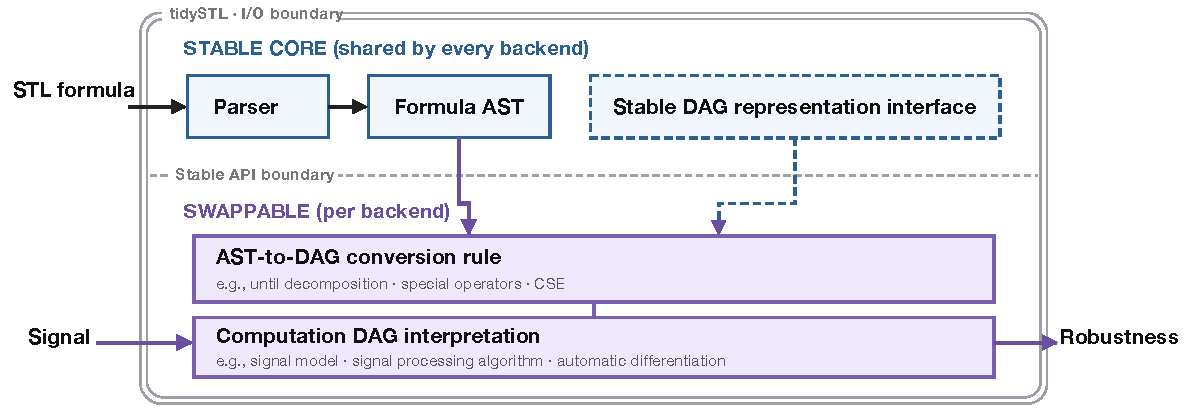
\includegraphics[width=\textwidth]{figures/architecture.pdf}
\caption{Architecture of \tool. The stable core (parser, formula AST, DAG
representation interface, public API) is shared by every backend; the
AST-to-DAG conversion rule and the DAG interpretation are swappable per
backend.}
\label{fig:arch}
\end{figure}

Internally, \tool separates a stable core from backend-specific evaluation logic, as shown in \cref{fig:arch}.
The stable core is shared by every backend, and it does not decide how $(\varphi, \sigma)$ maps to a robustness value.
Those decisions are delegated to the backend layer.


%\paragraph{Semantic choices vs.\ execution strategy.}
In the backend layer,
the \emph{semantic choices} fix what is computed: each backend resolves the decision points of \cref{tab:divergence} in a documented way, from the signal-interpretation choices of \cref{tab:siginterp} to extensions such as smooth aggregation~\cite{pant2017smooth}.
The \emph{execution strategy} fixes how it is computed: eager interpretation, batched vectorized evaluation, caching of shared nodes, or a future incremental schedule.

The separation is in service of \emph{observability}. When the formula
representation and the evaluation procedure are tightly coupled, as in most
existing tools, a suspicious robustness value is difficult to diagnose:
recovering which computation was actually performed means stepping through
evaluator internals. Keeping the semantic choices and the execution strategy
explicit makes the
computation traceable from the public API down to individual primitive
operations (the trace interface is documented in \cref{sec:app-trace});
the experiments in \cref{sec:discrepancies,sec:implement-variations}
revisit this point.

A backend realizes its choices in two steps: it lowers the formula AST into
a computation \emph{directed acyclic graph} (DAG) of typed primitive
operations, and it interprets
those operations into the chosen concrete signal-processing pipeline. The
lowering fixes the semantic choices and the interpretation fixes the
execution strategy, so semantics-preserving optimizations such as common
subexpression elimination and caching of shared nodes stay on the executor
side, never entangled with a semantic variant.
\cref{fig:inspectable-dag} illustrates the lowering on an example formula
with nested temporal operators.

\begin{figure}[t]
\centering
\begin{tikzpicture}[
font=\footnotesize,
box/.style={draw, rounded corners, align=center, inner sep=3pt},
group/.style={draw, dashed, rounded corners, inner sep=4pt},
grouplabel/.style={font=\footnotesize\itshape, anchor=south west},
arrow/.style={->, thick}
]

% ---- AST (root at top, leaves at bottom) ----
\node[box] (astG) {$\Box_{[0,5]}$};
\node[box, below=4mm of astG] (astAnd) {$\wedge$};
\node[box, below left=4mm and 1mm of astAnd] (astX) {$x \ge 0$};
\node[box, below right=4mm and 1mm of astAnd] (astF) {$\Diamond_{[0,2]}$};
\node[box, below=4mm of astF] (astY) {$y \ge 0$};

\draw[arrow] (astG) -- (astAnd);
\draw[arrow] (astAnd) -- (astX);
\draw[arrow] (astAnd) -- (astF);
\draw[arrow] (astF) -- (astY);

\node[group, fit=(astG) (astX) (astY)] (astgroup) {};
\node[grouplabel] at (astgroup.north west) {formula AST};

% ---- DAG (two rows, strict left-to-right flow) ----
% top row:    x -> Ineq -> Min -> WMin
% bottom row: y -> Ineq -> WMax (into Min)
\node[box, right=57mm of astAnd, yshift=9mm] (px) {\texttt{Ineq}\\ $p_x(t)$};
\node[box, below=5mm of px] (py) {\texttt{Ineq}\\ $p_y(t)$};
\node[box, right=6mm of py] (fwin) {\texttt{WMax}$_{[0,2]}$\\ $e_y(t)$};
\node[box] (andop) at (fwin |- px) {\texttt{Min}\\ $c(t)$};
\node[box, right=6mm of andop] (gwin) {\texttt{WMin}$_{[0,5]}$\\ $\rho_\varphi(t)$};

\node[left=4mm of px] (sx) {$x(t)$};
\node[left=4mm of py] (sy) {$y(t)$};

\draw[arrow] (sx) -- (px);
\draw[arrow] (sy) -- (py);
\draw[arrow] (px) -- (andop);
\draw[arrow] (py) -- (fwin);
\draw[arrow] (fwin) -- (andop);
\draw[arrow] (andop) -- (gwin);

\node[group, fit=(sx) (sy) (px) (fwin) (gwin)] (daggroup) {};
\node[grouplabel] at (daggroup.north west) {computation DAG};

% ---- lowering arrow between the groups (horizontal, at the height of astAnd) ----
\draw[arrow] (astgroup.east |- astAnd) -- (daggroup.west |- astAnd)
  node[midway, above=0.5mm, align=center] {backend-specific\\ lowering};

\end{tikzpicture}%

\caption{
Lowering of $\varphi :\equiv \Box_{[0,5]}\bigl((x \ge 0) \wedge
\Diamond_{[0,2]}(y \ge 0)\bigr)$ from the formula AST (left) to a
computation DAG (right). Nodes are typed primitive operations
(\texttt{Min} is pointwise; \texttt{WMax}/\texttt{WMin} aggregate over the
annotated window); edges carry the intermediate robustness signals, which
remain inspectable in the evaluation result.
}
\label{fig:inspectable-dag}
\end{figure}

\paragraph{Extension points.}

A backend consists of primitive operations, a lowering rule, and an executor.
Extensions may introduce new primitive operations during lowering or override the interpretation of existing ones.
Programming details are given in the user manual and reference implementations, both bundled with the \tool repository. \cref{sec:implement-variations} measures the code required for representative variants.

\paragraph{Implementation status.}
The implementation is open to new backends and primitive operations below the
stable core. The default backend supports  a future-time STL core over non-uniform time grids. Additional compatibility backends are demonstrated in
\cref{sec:discrepancies}.

% ------------------------------------------------

% ================================================================
\section{Evaluation}
\label{sec:evaluation}
% ----------------------------------------------------------------
%% Purpose of the section:
%% Show that tidySTL is useful as an evaluator layer:
%% (1) evaluator-level choices cause observable discrepancies;
%% (2) semantic and computational variations can be implemented locally
%%     under a common interface.
%% Experiment campaign plan: notes/eval-plan.md (experiments E1-E5).
% ================================================================

We evaluate \tool in two steps, one per claim. First, we show that
evaluator-level choices---the decision points of \cref{tab:divergence}---are
not cosmetic: across tools, they change robustness values, verdicts, trace
rankings, and downstream falsification and monitoring outcomes
(\cref{sec:discrepancies}). Second, we show that realizing such a choice in
\tool is a localized change below the stable interface, at measured
implementation cost and without undue overhead
(\cref{sec:implement-variations}).

% ================================================================
\subsection{Robustness Discrepancies Across Evaluator-Level Choices}
\label{sec:discrepancies}
% ----------------------------------------------------------------
%% Purpose:
%% Demonstrate that evaluator-level choices are not cosmetic:
%% they can change robustness values and downstream behavior.
%%
%% Figure/table:
%% - Cross-tool divergence matrix (real Breach/RTAMT/STLCG++), cells
%%   annotated with the decision points of tab:divergence; the
%%   baseline-agreement cells double as the validation claim       [E1]
%% - Divergence localization listing ("first divergent op")        [E2]
%% - Verdict-flip rates between named decision-point rules,
%%   swept over a trace family (monitoring consequence)            [E5b]
%% - Falsification performance under different objective semantics:
%%   falsifying rate + number of evaluations (ECDF over seeded
%%   repetitions); replaces the discarded objective-landscape plot  [E5a]
%% - Setting: same formula and signal, no special semantics
% ================================================================

Evaluator-level choices are the decision points of \cref{tab:divergence,tab:siginterp}: the questions an evaluator must answer but the formula does not. This subsection first establishes, using real-tool runs, that these choices produce observable robustness discrepancies. It then uses validated compatibility backends to localize the responsible choice and to illustrate downstream consequences. The experimental protocols and setup details are collected in Appendix~\ref{sec:app-eval}; the text here reports the findings.

\begin{table}[t]
\centering
\caption{Cross-tool divergence matrix: real Breach 1.11.4 (B), RTAMT 0.3.5
(R), and STLCG++ 0.0.2 with exact $\min$/$\max$ aggregation (S), compared
on per-timestep robustness at absolute tolerance $10^{-6}$ over a trace of
length $|\sigma|$. Per tool, $=$: matches the common behavior on the case;
$\ast$: differs from the other two tools; \mbox{--}: cannot express the
case (a coverage finding); $\dagger$: documented special handling (RTAMT
reads a non-uniform time grid as uniformly indexed samples). Each
diverging row names the responsible decision point of
\cref{tab:divergence,tab:siginterp}.}
\label{tab:divergence-matrix}
\small
% AUTO-GENERATED from extra/artifacts/rv2026-eval/e1/divergence_matrix.json
% by extra/experiments/e1_emit_matrix_tex.py (tidystl repo); do not hand-edit.
% B = Breach 1.11.4, R = RTAMT 0.3.5, S = STLCG++ 0.0.2 (hard min/max).
% Cells: = matches the common behavior (atol 1e-6, mutually defined
% timesteps), * differs from the other two, -- cannot express the case
% (coverage finding), dagger documented special handling.
\begin{tabular}{l c ccc l}
\hline
Case & $|\sigma|$ & B & R & S & Decision point \\
\hline
\multicolumn{6}{l}{\emph{Baseline block (operator coverage)}} \\
\quad $x \ge 3$ & 5 & $=$ & $=$ & $=$ &  \\
\quad $\neg (x \ge 0)$ & 5 & $=$ & $=$ & $=$ &  \\
\quad $(x \ge 0) \wedge (y \ge 0)$ & 5 & $\ast$ & $=$ & $=$ & terminal-step rule \\
\quad $(x \ge 0) \vee (y \ge 0)$ & 5 & $\ast$ & $=$ & $=$ & terminal-step rule \\
\quad $((x \ge 0) \wedge (y \ge 0)) \vee (z \ge 0)$ & 5 & $\ast$ & $=$ & $=$ & terminal-step rule \\
\quad $\Box_{[0,2]}(x \ge 0)$ & 5 & $=$ & $=$ & $=$ &  \\
\quad $\Box_{[1,2]}(x \ge 0)$ & 3 & $=$ & $\ast$ & $=$ & boundary rule \\
\quad $\Diamond_{[0,2]}(x \ge 0)$ & 5 & $=$ & $=$ & $=$ &  \\
\quad $\Diamond_{[1,3]}(x \ge 0)$ & 7 & $=$ & $\ast$ & $=$ & boundary rule \\
\quad $\Diamond_{[1,2]}(x \ge 0)$ & 3 & $=$ & $\ast$ & $=$ & boundary rule \\
\quad $(x \ge 0) \mathbin{U_{[0,3]}} (y \ge 0)$ & 5 & $=$ & $\ast$ & $=$ & open vs.\ closed endpoints \\
\quad $(x \ge 0) \mathbin{U_{[1,2]}} (y \ge 0)$ & 5 & $=$ & $\ast$ & $=$ & open vs.\ closed endpoints \\
\quad $(x \ge 0) \mathbin{U_{[0,4]}} (y \ge 0)$ & 5 & $=$ & $=$ & $=$ &  \\
\quad $(x \ge 0) \mathbin{U_{[1,2]}} (y \ge 0)$ & 2 & $=$ & $\ast$ & $=$ & boundary rule \\
\quad $x + y \ge 0$ & 4 & $=$ & $=$ & $=$ &  \\
\quad $x - y \ge 0$ & 4 & $=$ & $=$ & $=$ &  \\
\hline
\multicolumn{6}{l}{\emph{Divergence block (one case per decision point)}} \\
\quad $\Diamond_{[2,4]}(x \ge 0)$ & 3 & $=$ & $\ast$ & $=$ & boundary rule \\
\quad $(x \ge 0) \wedge (y \ge 0)$ & 3 & $\ast$ & $=$ & $=$ & terminal-step rule \\
\quad $\Box_{[0.5,1.5]}(x > 0)$ & 3 & $=$ & -- & -- & window alignment (coverage) \\
\quad $\Box_{[0,1]}(x > 0)$ & 5 & $=$ & $\dagger$ & -- & signal model \\
\quad $x = 3$ & 5 & $\ast$ & $=$ & $=$ & equality predicates \\
\hline
\end{tabular}%

\end{table}

\paragraph{Real-tool discrepancies.}
We first compare the original tools directly. Breach, RTAMT, and STLCG++
are run in their native environments on a shared case set, and their
per-timestep robustness outputs are compared at tolerance $10^{-6}$.
\cref{tab:divergence-matrix} summarizes the result: the baseline block
contains 16 operator-coverage cases from the regression suite, while the
divergence block isolates one evaluator-level choice in each of five
further cases.

The tools disagree even on small formulas and traces. In the baseline
block, one tool deviates from the other two on 9 of the 16 cases; most
disagreements come from Breach's terminal-step convention or RTAMT's
boundary rule for windows extending past the trace end. The divergence block isolates further
choices such as window alignment, signal model, and equality predicates.
The point is not that one tool is correct and another is wrong, but that
the same nominal input can induce different robustness behavior under
different evaluator-level choices.

\paragraph{Diagnosis by validated compatibility backends.}
The discrepancies themselves are established by running the original
tools. To inspect per-node traces and to name the responsible decision
point mechanically, we built compatibility backends for each tool; each
reproduces its tool's column of \cref{tab:divergence-matrix} per timestep
(62 of 63 case--tool cells agree; the one mismatch is deliberate and
documented). On a diverging case, a localizer reports the lowest
syntax-tree node whose per-node traces disagree: on the boundary-rule
headline row it returns \texttt{WindowMax[2,4]} vs.\
\texttt{DiscreteWindowMax[2,4]}, naming the boundary rule---requirement
R3 of \cref{sec:background} executed by the tool. The validation protocol
and the localization procedure are given in Appendix~\ref{sec:app-eval}.

\paragraph{Consequences beyond robustness values.}
The discrepancies are not knife-edge coincidences of single constructed traces.
Controlled trace sweeps show that the headline cases flip the verdicts a
monitor reports and the trace rankings a search acts on over intervals of
input values, not only at isolated points (sweep construction in
Appendix~\ref{sec:app-eval}).

\begin{figure}[t]
\centering
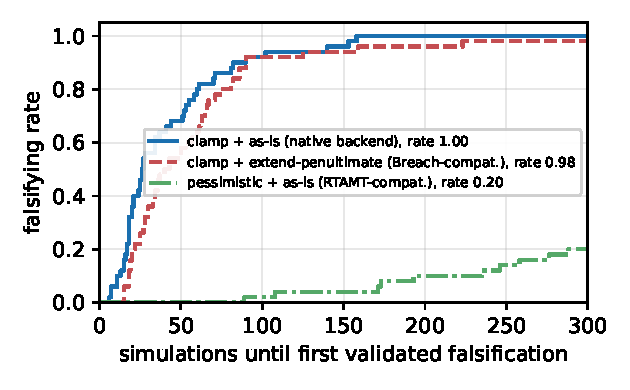
\includegraphics[width=.65\textwidth]{figures/falsification-ecdf.pdf}
\caption{Falsification performance under three objective semantics (named
boundary/terminal-step rule combinations, realized as \tool backends), with
the system, specification, search algorithm, seeds, and budget held fixed:
ECDF, over 50 seeded runs, of the number of simulations until the first
validated falsification (budget 300); the plateau height is the falsifying
rate. Candidate violations are validated by an exact system-level check, so
no backend acts as the verdict oracle.}
\label{fig:falsification}
\end{figure}

The same effect can compound downstream. We isolate this in a standard
falsification loop where the system, specification, search algorithm,
seeds, and budget are fixed, and only the objective semantics varies
across three boundary\slash terminal-step rule combinations: clamp with the
terminal step as-is, clamp with the extend-penultimate step, and
pessimistic with as-is (setup in Appendix~\ref{sec:app-eval}). The specification's monitor horizon reaches
past the end of the trace, so the boundary convention directly affects the
objective. \Cref{fig:falsification} shows the result: the clamping
variants falsify in 50/50 and 49/50 runs, while the pessimistic boundary
rule collapses the objective to the same out-of-range value for every
input and falsifies in only 10/50 runs.

This is not evidence that one boundary rule is globally inferior. The
collapse is a property of the pairing: a pessimistic boundary rule under a
whole-trace monitor objective. A user who knows this convention is in play
can restrict the monitor horizon and avoid the collapse. That is precisely
the point: compensating for an evaluator-level choice requires knowing
that the choice is there, and nothing in the optimizer's output reveals
it.

% ================================================================
\subsection{Implementing Evaluation Variations with Localized Changes}
\label{sec:implement-variations}
% ----------------------------------------------------------------
%% Purpose:
%% Show that tidySTL's layered design allows for semantic and computational variations
%% under a common interface, with changes localized to the evaluator layer.
%%
%% Figure/table:
%% - List of implemented variations with number of lines changed, regression tests. [E3]
%% - Performance results showing that variations do not cause undue overhead.
%%   (tab:scaling, extended with real RTAMT/STLCG++ baselines)      [E4]
%% - Performance results of tuned SIMD implementations.             [E3]
% ================================================================

% Appendix pointer:
% Regression suite details and expected-output generation.
% Tool-by-tool compatibility notes.
% Backend implementation notes.
% Additional benchmark results.

The previous subsection showed that evaluator-level choices have
observable consequences. We now measure the cost of realizing such choices
in \tool: how much code changes below the stable interface, and what
runtime overhead the explicit evaluator layer introduces.

\begin{table}[t]
\centering
\caption{Implemented variations. The key column is the layer changed; LOC
is reported only to make the locality claim auditable, not as a quality
metric (accounting rules in Appendix~\ref{sec:app-eval}). The full
regression suite passes with all variants installed.}
\label{tab:variation}
\footnotesize
% AUTO-GENERATED from extra/artifacts/rv2026-eval/e3/variation.json
% by extra/experiments/e3_emit_variation_tex.py (tidystl repo); do not hand-edit.
% LOC rule: variant-specific code only; blank/comment-only/docstring lines excluded; shared infrastructure excluded; attribution by top-level definition name (see script); Rust counted separately
% Full suite: 181 passed, 0 failed.
\setlength{\tabcolsep}{4pt}%
\begin{tabular}{l l r r}
\hline
Variant & Layer changed & LOC & Tests \\
\hline
\multicolumn{4}{l}{\emph{Semantic variants (what is computed)}} \\
\quad Breach-compatible & executor op overrides & 81 & 53 \\
\quad RTAMT-compatible & own lowering + executor & 191 & 20 \\
\quad STLCG++-compatible & own lowering + executor & 192 & 20 \\
\hline
\multicolumn{4}{l}{\emph{Computational variants (how it is computed)}} \\
\quad STLCG++ Torch executor & executor only & 241 & 3 \\
\quad Rust SIMD executor & executor only (native ext.) & 109 + 347 Rust & 26 \\
\hline
\end{tabular}%

\end{table}

\paragraph{Implementation effort.}
\cref{tab:variation} shows that the shipped variants change only
backend-side components. Semantic variants change primitive operations,
lowering rules, or executors below the stable core; computational variants
keep the semantics fixed and change only execution. Thus locality here
means a boundary of modification: the parser, formula representation,
signal layer, and user-facing interface are reused unchanged.

\begin{figure}[t]
\centering
% HAND-AUTHORED grouped bar plot of the data in figures/scaling-table.tex
% (auto-generated from extra/artifacts/rv2026-eval/e4/scaling_merged.json
% by e4_merge_scaling.py, tidystl repo). Update both together; the emitter
% does not yet produce this plot. Times in ms; RTAMT batched values are
% N x per-trace (dagger); STLCG++ OOMs at T=5001 (missing bars).
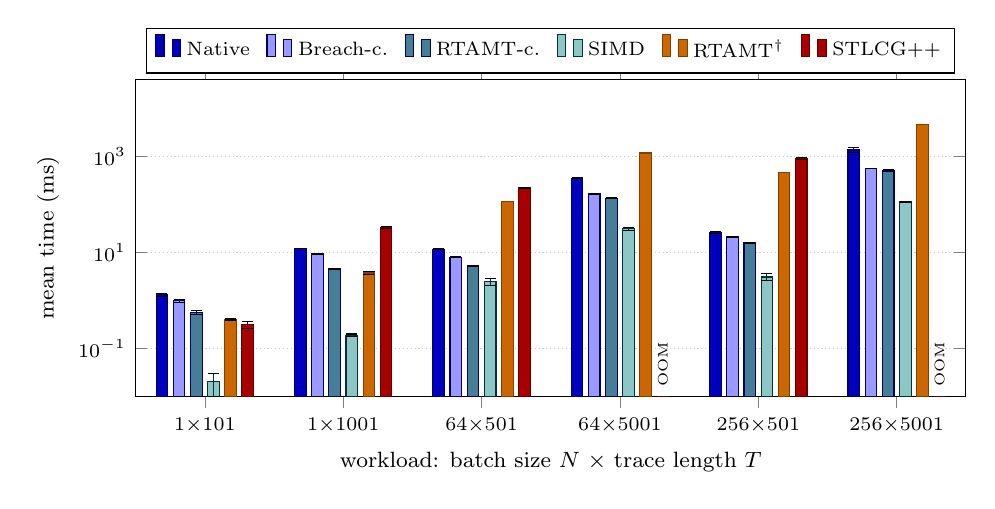
\begin{tikzpicture}
\begin{axis}[
  ybar,
  ymode=log,
  log origin=infty,
  width=\textwidth,
  height=5.6cm,
  bar width=4.2pt,
  ymin=0.01, ymax=40000,
  enlarge x limits=0.10,
  symbolic x coords={1x101,1x1001,64x501,64x5001,256x501,256x5001},
  xtick=data,
  xticklabels={
    {$1{\times}101$},{$1{\times}1001$},{$64{\times}501$},
    {$64{\times}5001$},{$256{\times}501$},{$256{\times}5001$}},
  xlabel={workload: batch size $N$ $\times$ trace length $T$},
  ylabel={mean time (ms)},
  legend columns=6,
  legend style={at={(0.5,1.02)}, anchor=south, font=\scriptsize,
    /tikz/every even column/.append style={column sep=4pt}},
  tick label style={font=\scriptsize},
  label style={font=\footnotesize},
  ymajorgrids,
  grid style={densely dotted, gray!40},
  error bars/y dir=both,
  error bars/y explicit,
]
% tidySTL backends (cool colors)
\addplot[fill=blue!75!black, draw=blue!40!black] coordinates {
  (1x101,1.30) +- (0,0.08) (1x1001,12.15) +- (0,0.19)
  (64x501,11.75) +- (0,0.25) (64x5001,358) +- (0,11)
  (256x501,26.19) +- (0,1.54) (256x5001,1377) +- (0,155) };
\addplot[fill=blue!40, draw=blue!40!black] coordinates {
  (1x101,0.98) +- (0,0.06) (1x1001,9.34) +- (0,0.28)
  (64x501,7.94) +- (0,0.15) (64x5001,167) +- (0,6)
  (256x501,21.42) +- (0,0.65) (256x5001,569) +- (0,9) };
\addplot[fill=cyan!55!black, draw=blue!40!black] coordinates {
  (1x101,0.57) +- (0,0.06) (1x1001,4.58) +- (0,0.08)
  (64x501,5.24) +- (0,0.20) (64x5001,136) +- (0,2)
  (256x501,15.97) +- (0,0.37) (256x5001,515) +- (0,23) };
\addplot[fill=teal!45, draw=teal!40!black] coordinates {
  (1x101,0.02) +- (0,0.01) (1x1001,0.19) +- (0,0.01)
  (64x501,2.44) +- (0,0.41) (64x5001,31.20) +- (0,1.89)
  (256x501,3.09) +- (0,0.50) (256x5001,115) +- (0,2) };
% real tools (warm colors)
\addplot[fill=orange!80!black, draw=orange!50!black] coordinates {
  (1x101,0.40) +- (0,0.01) (1x1001,3.74) +- (0,0.28)
  (64x501,118) (64x5001,1195) (256x501,471) (256x5001,4781) };
% OOM rows carry a zero-height phantom bar (y = ymin) whose node-near-coord
% prints the label exactly in the STLCG++ bar slot.
\addplot[fill=red!65!black, draw=red!40!black,
  point meta=explicit symbolic,
  nodes near coords,
  every node near coord/.append style={
    rotate=90, anchor=west, font=\tiny, text=black},
] coordinates {
  (1x101,0.31) +- (0,0.05) []
  (1x1001,33.71) +- (0,1.31) []
  (64x501,224) +- (0,3) []
  (64x5001,0.01) [OOM]
  (256x501,934) +- (0,44) []
  (256x5001,0.01) [OOM] };
\legend{Native, Breach-c., RTAMT-c., SIMD, RTAMT$^\dagger$, STLCG++}
\end{axis}
\end{tikzpicture}%

\caption{Mean evaluation time on representative workloads, plotted on a
log scale. All bars use the same formula
$\Box_{[0,5]}((x>0)\wedge\Diamond_{[0,2]}(y>0))$; error bars show one
standard deviation. RTAMT$^\dagger$ batch times are $N \times$ the
measured per-trace time; missing STLCG++ bars exceed memory (OOM). The
full timing table and benchmarking details are given in
\cref{tab:scaling}, Appendix~\ref{sec:app-eval}.}
\label{fig:scaling}
\end{figure}

\paragraph{Runtime cost.}
\cref{fig:scaling} compares \tool backends with real RTAMT and STLCG++ on
the same workload. On single traces, the explicit evaluator layer remains
within the same order of magnitude as the Python-stack references. On
batches, \tool's batch-first signal layout amortizes per-trace cost,
making the native backend substantially faster than looping RTAMT and
faster than the tensor-batched STLCG++ run shown here. The SIMD executor
gives the expected speed ceiling once per-node observability is dropped.
Thus the semantic and execution dimensions remain separable: the faster
executor changes how the native semantics is computed, not what semantics
is computed.

% ================================================================
\section{Related Work}
\label{sec:relatedwork}
% ----------------------------------------------------------------
% ================================================================

\cref{sec:background} already positions \tool against the main STL
tools. \tool differs from Breach, S-TaLiRo, RTAMT, and similar systems
not by replacing their workflows but by making the evaluator layer itself the
primary object of reuse~\cite{donze2010breach,donze2013efficient,annpureddy2011staliro,nickovic2020rtamt,nickovic2024rtamt}.

Proof-oriented monitoring work~\cite{dokhanchi2014online,chattopadhyay2020verified}
makes correctness guarantees for monitoring algorithms a central object.
\tool does not claim comparable formal verification; instead it makes
the semantic choices explicit so that divergence sources can be
identified without proof.

Speaking of implicitness is not a claim that tools such as RTAMT or Breach are
poorly documented. The choices in question are simply not determined by the
STL formula: adopting RTAMT, for instance, commits an evaluation to its
discrete-time signal and pessimistic boundary rule regardless of the
formula.
The ARCH-COMP 2021 report~\cite{ernst2021archcomp} documented cross-tool
discrepancies arising at exactly these decision points and
resolved them by post-hoc independent checking; \tool instead makes the
responsible choices explicit and switchable in advance.

MoonLight~\cite{bartocci2023moonlight} shows that pluggable monitoring domains
can be a first-class contribution; \tool applies the same lesson to the
semantic decision points of STL robustness evaluation.
TeSSLa, RTLola, and HLola~\cite{kallwies2022tessla,finkbeiner2019rtlola,sanchez2021hlola}
demonstrate that front-end/back-end separation is itself a scientific
contribution; their backends vary in execution platform while \tool's vary
in the semantic choices they realize.
STLCG and related differentiable tools~\cite{levenberg2020stlcg,kapoor2025stlcgpp} occupy the
smooth-semantics niche that the STLCG++-compatible backend in \tool targets
for comparison.


% ================================================================
\section{Conclusion and Future Work}
\label{sec:conclusion}
% ----------------------------------------------------------------
% ================================================================
\tool makes the semantic choices of STL robustness evaluation explicit at the evaluator boundary.  By separating formula syntax, signal data, backend-specific lowering, and DAG interpretation, it exposes choices that are otherwise buried in tool internals and shows that they materially affect verdicts, trace rankings, and falsification behavior across real, widely used tools---and that the choice responsible for a disagreement can be named mechanically.

The implementation supports the view of robustness evaluation as a reusable semantic layer rather than an implementation detail of a particular monitor, falsifier, or learning pipeline.  Semantic variants can be expressed by changing backend primitives, lowering rules, and DAG interpretations while preserving the public evaluation interface.  Future work will extend this layer to broader semantics, including online monitoring, and expand its validation suite.
